\chapter{Introduction}\label{chap:introduction}

\section{Structure of the thesis}
The objective of this work is to explore observational evidence and indirect detection of dark matter, and to review the quantum-mechanical effect known as Sommerfeld enhancement \cite{Sommerfeld_1931}, particularly to understand how its presence can deeply affect the theoretical predictions of some relevant dark matter models. This will be done by considering the theoretical framework laid out by Arkani-Hamed et al. in \cite{Arkani_2009} and by applying it to the experimental limits on the dark matter annihilation cross section found by Profumo et al. \cite{Profumo_2018} through direct observation of gamma-ray production from dwarf spheroidal galaxies orbiting the Milky Way. The thesis is structured in three parts:
\begin{itemize}
	\item In Chapter \ref{chap:introduction}, I introduce the concept of dark matter together with an overview of evidence for its existence and an explanation of its indirect detection. At the end of the chapter, a detailed description of Sommerfeld enhancement and its use in this work will be given.
	\item In Chapter \ref{chap:derivation}, I will thoroughly explain the mathematical derivation that leads to the final expression of the Sommerfeld enhancement factor in the so-called Coulomb approximation.
	\item In Chapter \ref{chap:implications}, I will apply the concepts and formulae set out in the first two chapters to derive lower bounds on the dark matter mass with and without Sommerfeld enhancement. After this, I will check whether the Coulomb approximation was a good approximation in this case, and I will draw the conclusions of this research.
\end{itemize}

The whole thesis uses natural units where \(c=\hbar=1\). Numerical calculations had to be performed to compute the enhanced cross section: for completeness, the code I wrote is open-source on \href{https://github.com/LuckeeDev/bachelor-thesis}{GitHub}.

\section{Dark matter}

I will now try to give an overview of the history of dark matter, which problems it solves and an account of the main pieces of cosmological and astrophysical evidence supporting its existence. Most of the content of this section comes from the following sources, which I recommend to the reader to delve deeper into how dark matter has come to be accepted as part of the standard cosmological model: \emph{History of dark matter} by Bertone and Hooper \cite{Bertone_2018}, an excellent rundown of historical developments in the research on this topic which credits the contributions of way more researchers than those that I'll report in the following; \emph{Dark matter} by Cirelli, Strumia and Zupan \cite{Cirelli_2024}, the most complete review on dark matter to date; and the lectures given by Volansky in Florence in 2014 \cite{Volansky_2014} and by Lisanti in Trieste in 2018 \cite{Lisanti_2018}.

\subsection{Galaxy clusters}

Hints of new physics come from all cosmological scales. Historically, the first to arise were on the scale of galaxy clusters with Zwicky's research about Coma cluster's velocity dispersion in 1933 \cite{Zwicky_1933}. He first applied the virial theorem to estimate the velocity dispersion of galaxies in the Coma cluster. For a gravitationally-bound system in equilibrium, the virial theorem states that the time-averaged kinetic energy of the system \(\langle T \rangle \) is equal to the opposite of half of the time-averaged total potential energy \(\langle U \rangle \) of the system:
\begin{equation}\label{eq:diff_potential}
	\langle T \rangle = - \frac{1}{2} \langle U \rangle 
\end{equation}
In order to reproduce Zwicky's calculations, I will assume Coma to be a homogenous sphere of mass \(M\) and radius \(R\). The potential energy between a shell of thickness \(\mathrm{d} r\) at radius \(r\) and the interior of the shell is
\begin{equation}
	\mathrm{d} U = - G \frac{M_{shell} M_{int} }{r}
\end{equation}
where
\begin{equation}
	M_{shell} = 4\pi \rho r^2 \mathrm{d} r
	\qquad
	M_{int } = \frac{4}{3} \pi \rho r^3
\end{equation}
where \(\rho \) is the density of the cluster. The total potential energy is found by integrating Eq. \eqref{eq:diff_potential} from \(0\) to \(R\) and is
\begin{equation}\label{eq:shell_potential}
	\langle U \rangle = \int\limits_0^R \mathrm{d} U = - \frac{3GM^2}{5R}
\end{equation}
We now assume that the cluster is made up of \(N\) galaxies of equal mass \(m\). This gives a total kinetic energy of
\begin{equation}\label{eq:kinetic}
	\langle T \rangle = \frac{1}{2} Nm \langle v^2 \rangle 
\end{equation}
Applying the virial theorem gives a velocity dispersion of
\begin{equation}\label{eq:dispersion}
	\sqrt{\langle v^2 \rangle } = \sqrt{\frac{3GNm}{5R}} \simeq 82 \mathrm{km / s}, 
\end{equation}
where I have used Zwicky's estimates of \(N=800\) galaxies of \(m = 10^9 M_\odot\) in a sphere of radius \(R=10^6 \mathrm{ly} \) \cite{Bertone_2018}. This result is off by orders of magnitude from the line-of-sight velocity dispersion of visible matter in the Coma cluster measured via Doppler redshifts today, which is \(v_{los} \sim 10^3 \mathrm{km /s} \).
% TODO: find reference for v_los and other Coma data

The discrepancy in the velocity dispersion could be explained by an additional component of dark matter mass in the cluster. In order to show this, I am going to perform the same calculation as above, but starting from the known velocity dispersion to give an estimate of the cluster's mass. We know that Coma is \(\sim 100 \mathrm{Mpc} \) away from us, that it occupies an angular radius of order \(1\) degree and that it is approximately spherically symmetric. By inverting Eq. \eqref{eq:dispersion}, we find that
\begin{equation}
	M= \frac{5R \langle v^2 \rangle }{3G} = \frac{5R v_{los} ^2}{G},
\end{equation}
where I have assumed that the velocity is isotropic and therefore \(\langle v^2 \rangle = 3 v_{los} ^2\). The radius of the cluster can be found from its distance from Earth and its angular radius:
\begin{equation}
	\frac{R}{d} \simeq 1^{\circ} = \frac{\pi}{180}
\end{equation}
which gives a mass of
\begin{equation}
	M=\frac{\pi}{36} \frac{d v_{los} ^2}{G} \simeq 2 \times 10^{15} M_\odot
\end{equation}
This estimate is off by one order of magnitude compared to the estimate of \(10^{14} M_\odot\) coming from the visible mass in its galaxies and the mass in gas measured from its X-ray emission. This suggests that a large part of mass in the Coma cluster is currently unaccounted for.

\subsection{Galactic rotation curves}\label{sec:rotation_curves}
Another important piece of evidence followed in 1970 with Rubin and Ford's optical observations of the M31 galaxy rotation curves \cite{Rubin_1970}. It had been known for a long time that Andromeda rotates, but their measurements represented a significant improvement on previous ones and hinted for the first time at an unexpected velocity distribution in the outskirts of the galaxy. From Newtonian mechanics, we expect the rotational velocity at a distance \(r\) from the centre of the disk to be related to the enclosed mass \(M(r)\) by \cite{Lisanti_2018}
\begin{equation}\label{eq:rotational_velocity}
	v(r)=\sqrt{\frac{GM(r)}{r}} 
\end{equation}
Assuming a typical exponential mass distribution, Freeman \cite{Freeman_1970} derived a decaying velocity curve at large radii that is shown in Fig. \ref{fig:rotation_curves}. Surprisingly, Rubin and Ford's data seemed to flatten out at large radii. This was confirmed shortly after by studies conducted with 21cm HI line observations, which allowed to extend the data further out into the galactic disc. These studies are summarised in Fig. \ref{fig:rotation_curves}: the pink markers show the first attempt at determining the galaxy's rotation curve by Babcock in 1939 \cite{Babcock_1939}; the black dots show the above-mentioned data from Rubin and Ford with optical observations; the red points and green points are 21cm HI line measurements, from Roberts and Whitehurst in 1975 \cite{Roberts_1975}, and Carignan et al. in 2006 \cite{Carignan_2006} respectively. Similar observations have been made for many other galaxies and have been collected by Bosma in \cite{Bosma_1981}.
\begin{figure}[!ht]
	\centering
	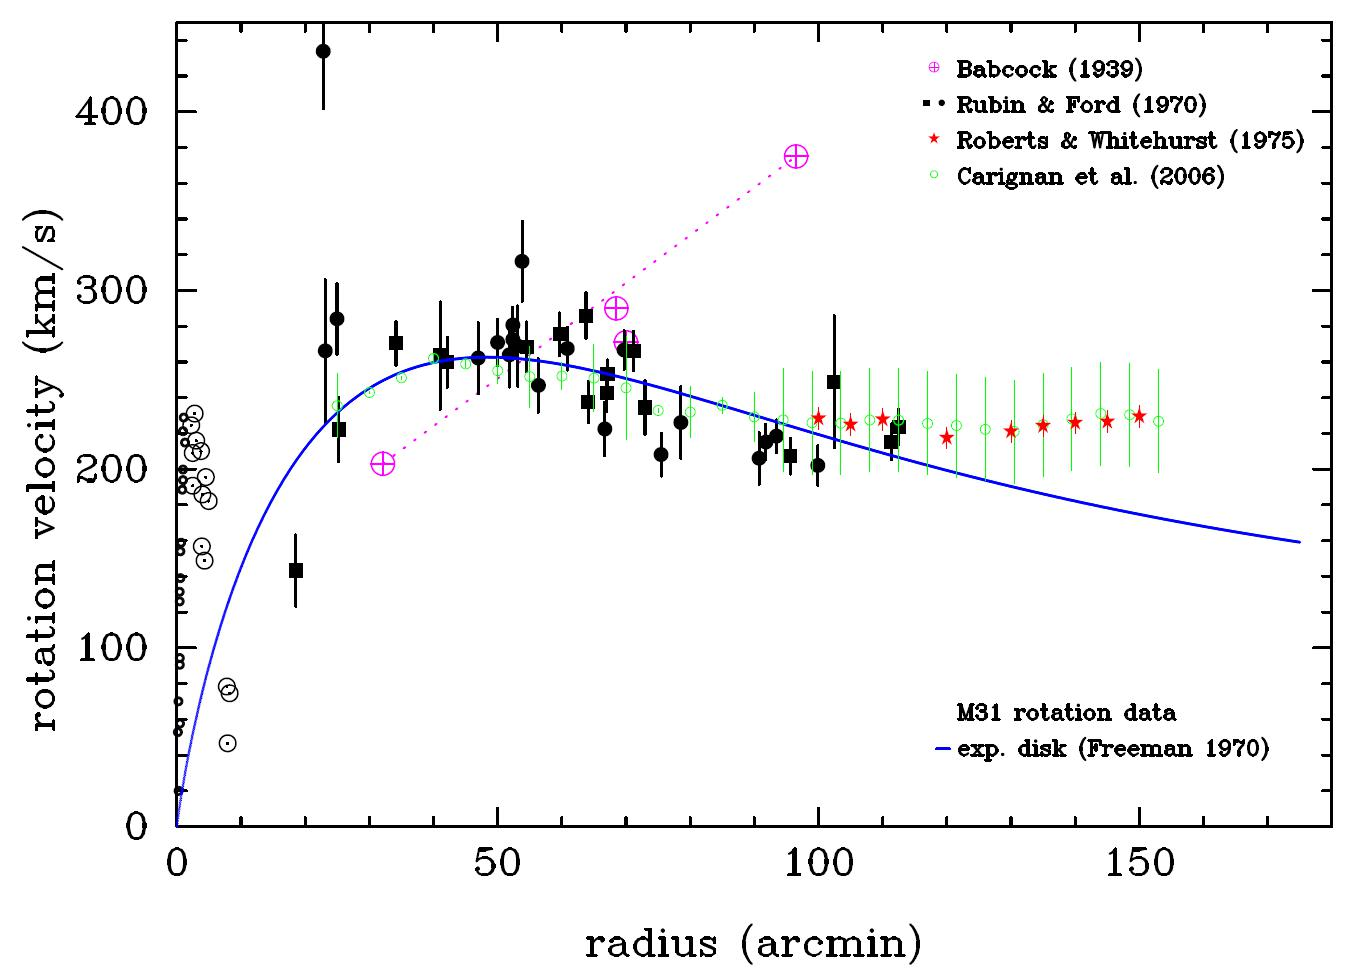
\includegraphics[width=0.8\textwidth]{rotation_curves.jpg}
	\caption{Rotational velocity data points for the M31 galaxy from several sources \cite{Babcock_1939, Rubin_1970, Roberts_1975, Carignan_2006}. The solid blue line represents the expected velocity curve in the hypothesis of an exponential mass distribution \cite{Freeman_1970}. Credits for the figure: Albert Bosma.}
	\label{fig:rotation_curves}
\end{figure}

Two approaches have been attempted to solve this issue: the first one, known as Modified Newtonian Dynamics (MOND), sets out to adjust Newton's second law to explain the discrepancies in observational data, but has struggled to gain consensus and has been partially ruled out by evidence outlined in Section \ref{sec:bullet}. The second one, currently accepted by the scientific community, is the presence of additional dark matter inside galaxies.
By inspecting Eq. \eqref{eq:rotational_velocity}, we can infer that \(v(r)\) would flatten in the case of \(M \propto r\), or in other words \(\rho \propto r^{-2} \) in the hypothesis of a spherically-distributed dark matter ``halo''\footnote{The hypothesis of the existence of these spherical ``halos'' is well-motivated, because as we will see later dark matter is non-dissipative and thus does not collapse to form a disk.}. The precise dark matter distribution can be derived from numerical simulations, which however strongly depend on the assumptions used to construct them. One of the most common profiles used in the literature, and also by Profumo et al. in the reference paper for this work \cite{Profumo_2018}, is the so-called Navarro-Frenk-White profile
\begin{equation}\label{eq:NFW}
	\rho_{\text{NFW}} (r) = \frac{\rho _s}{\frac{r}{r_s}\left( 1+ \frac{r}{r_s} \right)^2 },
\end{equation}
where \(\rho _s\) and \(r_s\) are scale parameters to be determined.

\subsection{The Bullet cluster}\label{sec:bullet}
The so-called Bullet cluster constitutes, together with the Cosmic Microwave Background (CMB) \cite[Section 1.3]{Cirelli_2024}, the strongest piece of evidence against MOND and in favor of dark matter. The findings were presented by Clowe et al. in 2006 \cite{Clowe_2006} as \emph{a direct empirical proof of the existence of dark matter}. The idea behind the paper was to use gravitational lensing to map the gravitational potential of the cluster and compare it to the X-ray image of the system. When the two clusters shown via a colormap in Fig. \ref{fig:bullet} collided, the dissipationless galaxies and stars spatially separated from the hot X-ray emitting gas. As the gas is the dominant baryonic mass component, one would expect the gravitational potential to loosely trace its distribution, however, as one can see from the green contours, the centre of mass of the system is severely displaced from that of the gas. This suggests that most of the matter in the system is actually unseen and, like galaxies and stars, it has not interacted during the collision.

\begin{figure}[!ht]
	\centering
	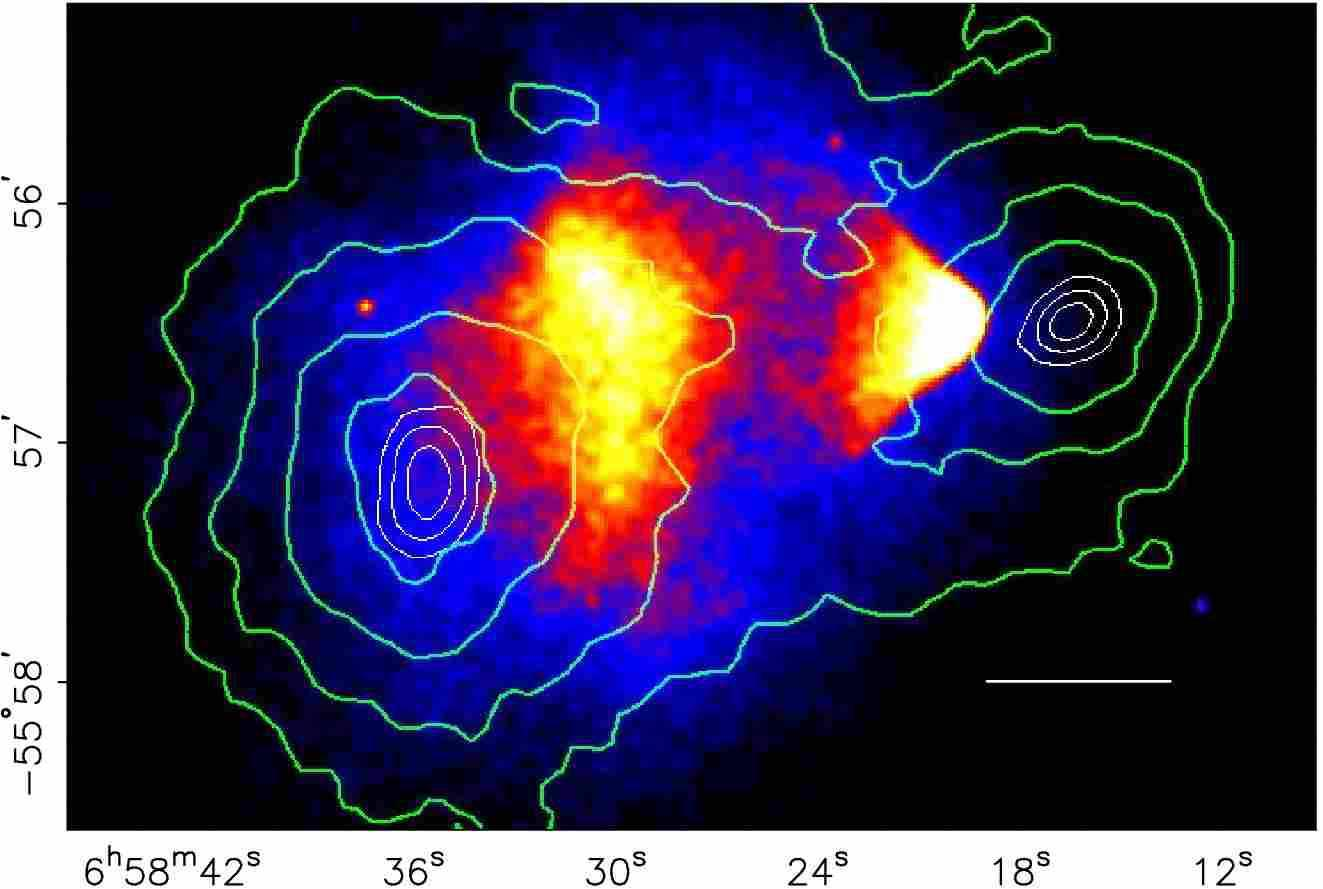
\includegraphics[width=0.8\textwidth]{bullet.jpg}
	\caption{The Bullet cluster. The colormap shows the distribution of X-ray emitting mass in the system. The green contours show the reconstructed gravitational lensing signal. The white bar is for scale and represents a distance of \(200 \mathrm{kpc} \) at the location of the cluster. Credits for the figure: Clowe et al. \cite{Clowe_2006}.}
	\label{fig:bullet}
\end{figure}

\subsection{The properties of dark matter and WIMPs}

The plethora of astrophysical and cosmological data gathered about dark matter can be summarised by saying that we expect dark matter to be \emph{cold, non-interacting matter with adiabatic inhomogeneities} (Cirelli et al., \cite[Chapter 1]{Cirelli_2024}). \emph{Cold} refers to the fact that dark matter behaved as a non-relativistic fluid at the time of matter-radiation equality, and this allowed it to cluster and form structures like the ``halos'' mentioned in Section \ref{sec:rotation_curves}. \emph{Non-interacting} is what makes dark matter so hard to detect: it means that dark matter's interactions with any other kind of matter can be \emph{cosmologically} neglected. This does not mean that dark matter does not interact at all: indirect detection, which will be further discussed in Section \ref{sec:indirect_detection}, relies on dark matter annihilating with itself and producing detectable astrophysical signals. \emph{Stable} means that it has existed since the beginning of the universe and that it has not disappeared yet, while \emph{adiabatic} means that the composition of the dark matter fluid is homogeneous on cosmological scales. The description given by Cirelli et al. also stresses the word \emph{matter}, because we expect its density to be proportional to the inverse of the volume (contrary to dark energy, whose density seems to remain constant at any scale).

Weakly Interacting Massive Particles (WIMPs) are a strong candidate for dark matter that satisfy all of these conditions. They have been the most studied dark matter candidate so far, and in particular they constitute the object of research of the reference work by Profumo et al. \cite{Profumo_2018}, that will be used later in this thesis.
Despite suggesting a connection with the weak interaction, the term is used more broadly in the paper, and means a class of particles that has interactions with strength on the scale of the weak interaction, and thus has weak-scale-like annihilation cross section and mass. One of the main points of interest about WIMPs is that they could easily explain today's dark matter abundance via a thermal freeze-out process as described in detail in \cite[Chapter 4]{Cirelli_2024}. Briefly, this would mean that dark matter and standard model particles were once part of the same interacting thermal bath, but that at one point the temperature dropped below a certain threshold so that the dark matter stopped interacting and decoupled from the bath. The dark matter that exists today is a ``relic'' from this frozen process. Coincidentally, the required cross-section that one obtains by working in this theoretical framework is of the order of a typical weak-scale annihilation cross section (this is commonly referred to as the \emph{WIMP miracle}).

\section{Indirect detection}\label{sec:indirect_detection}
Indirect detection experiments aim at detecting an excess of cosmic ray fluxes due to dark matter above expected astrophysical contributions. This can happen if dark matter annihilates or decays to standard model particles that then travel to Earth and can be detected by telescopes. This comes with its own significant challenges, given especially by the high astrophysical background. Despite this, some of the stricter bounds on dark matter annihilation cross section today \cite{Hooper_2018} come from this kind of experiments and by works like \cite{Profumo_2018}. In the following, I will show how the gamma-ray flux on Earth depends on the dark matter's properties and on the astrophysical properties of the object in study. This will be used to briefly discuss potential targets for indirect detection. Later, I will show how the hypotheses that we set on the dark matter distribution can greatly impact the interpretation of the gamma-ray flux.

\subsection{Gamma-ray flux from dark matter annihilation}
In order to compute the contribution to gamma-ray fluxes from dark matter annihilation, I will start by counting the number of possible annihilating pairs in a volume \(\mathrm{d}^3 \vec{r}\). In the hypothesis of non-self-conjugate dark matter, this number is
\begin{equation}\label{eq:dN}
	\mathrm{d} N = \frac{1}{4} \left( \frac{\rho_{DM} (\vec{r})}{M_{DM} } \right) ^2 \mathrm{d}^3 \vec{r}
\end{equation}
This is because annihilation is a two-body process, and the number of pairs is proportional to the square of the number of particles. The gamma-ray flux due to dark matter decay can be obtained in a similar fashion by using instead a linear proportionality, since it is a one-body process. A factor of \(1 /2\) is introduced to avoid counting pairs twice, and another one comes from the fact that each particle can only annihilate with half of the total number of particles because they are non-self-conjugate \cite{Sala_2019}.

Assuming that dark matter annihilates into a pair of standard model particles \(f\) with cross section \(\langle \sigma v \rangle_f \), then multiplying Eq. \eqref{eq:dN} by \(\langle \sigma v \rangle_f \) and summing over all possible decay products gives the total number of dark matter annihilations per second:
\begin{equation}
	\frac{\mathrm{d}N}{\mathrm{d}t} = \mathrm{d} ^3 \vec{r} \frac{1}{4} \left( \frac{\rho_{DM} (\vec{r})}{M_{DM} } \right)^2 \sum_{f} \langle \sigma v \rangle_f
\end{equation}

We can get the rate of photons produced per second per energy unit by multiplying by the number of photons produced by the species \(f\) inside the sum:
\begin{equation}
	\frac{\mathrm{d}N_{\gamma } }{\mathrm{d}t \mathrm{d} E} = \mathrm{d} ^3 \vec{r} \frac{1}{4} \left( \frac{\rho_{DM} (\vec{r})}{M_{DM} } \right)^2 \sum_{f} \langle \sigma v \rangle_f \frac{\mathrm{d}N_{f \to \gamma } }{\mathrm{d}E}
\end{equation}

To get the differential flux of photons per unit energy and per unit angle at the detector, we integrate over the line of sight \(s\) by writing the volume element as \(\mathrm{d} ^3 \vec{r}= s^2 \mathrm{d} s \mathrm{d} \Omega \). The integrand must be weighed by the distance factor \((4\pi s^2)^{-1} \):
\begin{equation}\label{eq:flux_per_energy}
	\frac{\mathrm{d}\Phi_{\gamma } }{\mathrm{d}E \mathrm{d} \Omega } = \int\limits_{los} \frac{1}{16\pi }\left( \frac{\rho_{DM} (\vec{r})}{M_{DM} } \right)^2 \sum_{f} \langle \sigma v \rangle _f \frac{\mathrm{d}N_{f\to \gamma } }{\mathrm{d}E} \mathrm{d} s,
\end{equation}
where \(\Phi_{\gamma } \) is the integrated gamma-ray flux, typically expressed in units of \(\mathrm{cm^{-2} s^{-1} sr^{-1} } \). All the astrophysical information can be summarised by defining the so-called J-factor, which in the specific case of the Milky Way is
\begin{equation}
	J(\theta ) = \int\limits_{los} \frac{\mathrm{d}s}{r_\odot} \left( \frac{\rho_{DM} (s, \theta )}{\rho_\odot} \right)^2,
\end{equation}
which allows us to rewrite Eq. \eqref{eq:flux_per_energy} in the following form:
\begin{equation}
	\frac{\mathrm{d}\Phi_{\gamma } }{\mathrm{d}E \mathrm{d} \Omega }(\theta ) = \frac{1}{4} \frac{r_\odot}{4\pi }\left( \frac{\rho_\odot}{M_{DM} } \right)^2 J (\theta ) \sum_{f}  \langle \sigma v \rangle _f \frac{\mathrm{d}N_{f\to \gamma } }{\mathrm{d}E}, 
\end{equation}
where \(\theta \) is the aperture angle from the centre of the galaxy, \(r_\odot\) is the distance of the sun from the centre of the Milky Way, \(\rho_\odot\) is the local dark matter density, and \(s\) is related to \(r\) by the relation \(r=\sqrt{r_\odot^2 + s^2 - 2 r_\odot s \cos \theta } \). We are often interested in the gamma-ray flux integrated over a region that spans a spherical angle \(\Delta \Omega \). In this case, we define the averaged J-factor, which for an annulus centred around the galactic centre with \(\theta_{min }< \theta < \theta_{max} \) is \cite{Cirelli_2024}
\begin{equation}
	\overline{J} = \frac{2\pi }{\Delta \Omega } \int\limits_{\theta_{min}}^{\theta_{max} }\sin \theta J(\theta ) \mathrm{d} \theta 
\end{equation}

Inspecting the form of the averaged J-factor leads us to identify four main characteristics of promising indirect detection targets \cite{Hooper_2018}:
\begin{enumerate}
	\item High density of dark matter
	\item Proximity to us
	\item Extended across a large volume
	\item Accompanied by a low astrophysical background
\end{enumerate}
Dwarf spheroidal galaxies (dSphs) are particularly interesting because of the last point, despite having rather small J-factors compared to the galactic centre. Therefore, in order to get reliable data from dSphs, years of observations must be collated and stacked analysis of multiple dSphs must be performed. This is what Profumo et al. did in \cite{Profumo_2018}.

\subsection{Impact of J-factor on cross section estimates}
The assumed dark matter profile, which enters in the flux calculation through the J-factor, can severely impact the dark matter annihilation cross section bounds. This can be shown by a simple numerical calculation. I am going to compare two different dark matter profiles: a spiked NFW profile like that in Eq. \eqref{eq:NFW}, and a cored one:
\begin{equation}
	\rho_{\text{NFW}}^{\text{core} } = \rho _s \frac{r_s}{r+ r_0} \frac{1}{\left( 1 + \frac{r}{r_s} \right) ^2}
\end{equation}
I am going to use the following parameters taken from Balaji et al. \cite{Balaji_2023} with reference to the Milky Way: \(r_s = 18.6 \mathrm{kpc}, \rho_\odot = 0.383 \mathrm{GeV / cm^3}, r_\odot = 8.2 \mathrm{kpc}  \) and \(\rho _s = \rho _\odot (r_\odot / r_s) (1 + r_\odot / r_s)^2\). For the cored profile, I will assume the core to have a size of \(r_0 = 0.5 \mathrm{kpc} \). With reference to the work by the H.E.S.S. collaboration in 2016 \cite{Abdallah_2016}, I computed the averaged J-factor over the annulus \([0.3^\circ, 1.0^\circ]\) (see \href{https://github.com/LuckeeDev/bachelor-thesis}{GitHub} for the code):
\begin{equation}
	\overline{J}_{\text{NFW} } \simeq 1100
	\qquad
	\overline{J}_{\text{NFW} }^{\text{core} } \simeq 100   
\end{equation}
Since for a given gamma-ray flux \(\langle \sigma v \rangle \propto \overline{J}^{-1} \), we can see that bounds on the cross section can vary by up to an order of magnitude depending on the choice of the dark matter profile. In particular, bounds with a NFW profile will be stricter compared to those with a cored NFW profile.

\section{Sommerfeld enhancement}

Initially studied by Sommerfeld in 1931 \cite{Sommerfeld_1931}, the Sommerfeld enhancement is an effect arising in non-relativistic quantum mechanics where the introduction of a long-range potential affects the cross section of a process happening locally at the origin.

One can easily picture the effect by making an analogy with classical mechanics. Consider an object traveling with velocity \(v\) towards a star of radius \(R\) and mass \(M\): if we neglect gravity, the cross section for falling into the star is simply the area occupied by the star \(\sigma _0=\pi R^2\). However, if we consider gravity, the cross section increases because the object can be dragged from further away into the star. This means that the cross section is actually \(\sigma = \pi b_{max}^2 \), where \(b_{max}\) is the largest the impact parameter can be for the distance of closest approach of the orbit to be \(R\) \cite{Arkani_2009, Cirelli_2024}. We can determine the enhancement factor by imposing conservation of energy and angular momentum, and get
\begin{equation}
	\sigma = \sigma _0 \left( 1+ \frac{v_{esc} ^2}{v ^2} \right), 
\end{equation}
where \(v_{esc} ^2 = 2GM / R\) is the squared escape velocity from the surface of the star. The cross section can thus be greatly enhanced at velocities \(v \ll v_{esc} \).

In quantum mechanics, something similar can happen with the introduction of a long-range potential. Consider, for instance, an annihilation happening locally at the origin thanks to a Hamiltonian of the type \(H_{ann} = U_{ann} \delta (\vec{r})\). The rate of the process will be proportional to the squared modulus of the wavefunction at the origin \(\vert \psi ^{(0)}(0) \vert^2 \). If we introduce a potential, the original wavefunction will get distorted and will have a different value at the origin, now making the rate proportional to \(\vert \psi (0) \vert^2 \). The Sommerfeld enhancement factor is defined as the ratio between the two cross sections, and therefore between the squared moduli of the wavefunctions:
\begin{equation}\label{eq:sommerfeld_def}
	S = \frac{\sigma }{\sigma _0} = \frac{\vert \psi (0) \vert ^2}{\vert \psi ^{(0)}(0) \vert ^2}
\end{equation}

Although dark matter does not interact electromagnetically and gravity is irrelevant at these scales, Sommerfeld enhancement can be extremely relevant for dark matter theory in the hypothesis that the dark matter particles couple to an attractive force carrier with Compton wavelength longer than \((\alpha M_{DM})^{-1} \), where \(\alpha\) is the strength of the interaction and \(M_{DM} \) is the mass of the dark matter particle. In other words, we're referring to a light force carrier \(\phi \) with mass \(m_{\phi } \lesssim \alpha M_{DM} \). This light force carrier could be the mediator of a yet unknown ``dark interaction'': this claim exists in several theories of physics beyond the standard model \cite{Arkani_2009}.

Since the mediator is expected to be massive, the most natural way to model the long-range interaction would be a classic Yukawa potential:
\begin{equation}
	V(r) = -\frac{\alpha }{r} e^{-m_{\phi } r}
\end{equation}
However, in the limit of a massless mediator, the potential tends to a simple Coulomb potential and the associated Schrödinger equation admits an analytic solution. Intuitively, one can make the approximation of a massless mediator, and thus an infinite-range force, when the range of the force is larger than the De Broglie wavelength of the system \((\mu v_{rel})^{-1} \), where \(\mu \) is the reduced mass and \(v_{rel} \) is the relative velocity of the two particles \cite{Sala_2019}. This translates into the following constraint for two particles with identical mass \(M_{DM} \):
\begin{equation}
	\frac{M_{DM} v_{rel} }{2m_{\phi } }\geq 1
\end{equation}
If the Coulomb approximation is not valid, one should instead use the Yukawa potential and solve the equation numerically, or else approximate it with the Hulthen potential to be able to solve the problem analytically:
\begin{equation}\label{eq:Coulomb_approx}
	V_H(r) = -\alpha \kappa m_{\phi } \frac{e^{-\kappa m_{\phi }r }}{1- e^{-\kappa m_{\phi }r }},
\end{equation}
where the approximation is most accurate for \(\kappa \thickapprox 1.74\) \cite{Cirelli_2024}. In the following, I will always assume a massless mediator, and I will later check if it was indeed a good approximation.

One more reason for being interested in Sommerfeld enhancement is that, as we will see in the following, it is velocity-dependent, and therefore allows for different cross sections at freeze-out and today. In particular, it allows higher cross sections today compared to the one that is required to give the correct dark matter thermal relic abundance (\(\langle \sigma v \rangle_{relic}=4.4\times 10^{-26} \mathrm{cm^3 s^{-1}}\) for non-self-conjugate dark matter \cite{Hooper_2018}).